\documentclass{article}


\usepackage[utf8]{inputenc}
\usepackage[english]{babel}
\usepackage{biblatex}
\usepackage{graphicx}
\usepackage{mathbbol}
\addbibresource{biblio.bib}
\bibliography{biblio}


\title{Visualisation of big knowledge graphs}
\author{Flora Helmers, Mahsa Niazi}
\begin{document}
\maketitle

\section*{Introduction}
Posing the problem:
huge graphs 
visualisation (limits of 2D)



Increasing number of datasets made out if graphs : DBpedia, ....

Some languages enable to query them like Sparql. 

Not accessible to many people (need to connect to the endpoint , and query the language. 

But the principal is quite simple : each entity can be linked to another by a predicate. For example in the linkedimdb there are 85k+ movies with the links between actors and realisator. 
What is interesting would be to explore the nodes and their connexions on an interactive map. It would help for instance to visualize better.

So the goal is to create a visually pleasing graph on a 3D. 
3D is not often used in visualisation, as it doesn't facilitates the sharing of the picture. But since we have polyscope at our disposal it helps to generate easily a 3D map. 

Many algorithms exist to draw graphs in 2D. But far less exist to draw large graphs in 3D. Therefore we use the GRIP algorithm proposed by Gajer and Kobourov in \cite{gajer00}.that was conceived for graphs of size 30k nodes.  


\section{Structure of the code}

\begin{figure}[h!]
    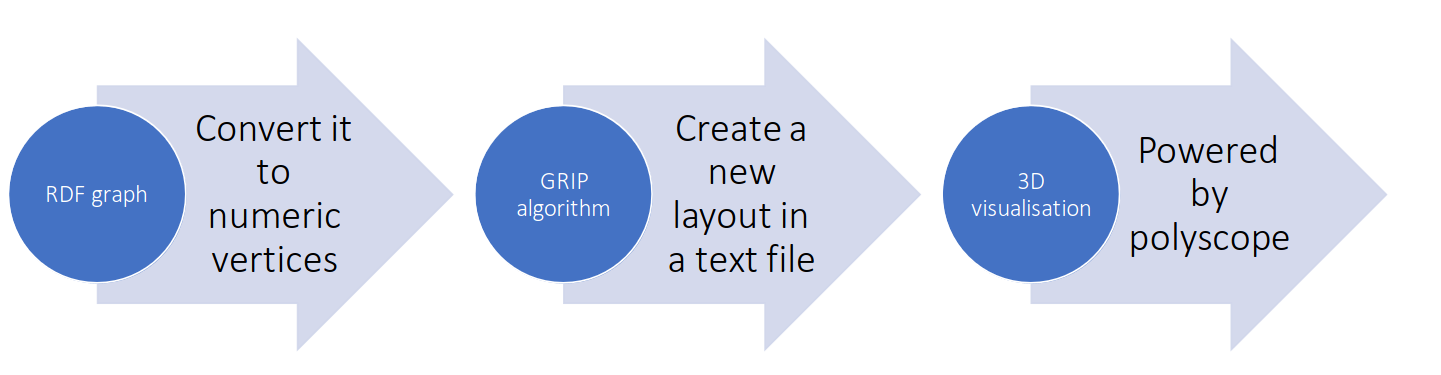
\includegraphics[width=\textwidth]{process.png}
    \caption{Overview of the process}
\end{figure}

The original format of the file is the one of the knowledge graph, which is a triple (subject, object, predicate). There exist many serialisation format to express these triples. But for us, it means that the construction of the graph will be at least linear in the number of triple. Small datasets are made of less than 100k triples. Transforming it in the numeric format is possible, if we put the limit of INT\textunderscore MAX, else we could consider using the type double. We store the graph in the form of adjacency lists. If there are several edges between a pair of vertices, we consider them has being one, because we can play on this parameter afterward in the visualisation. 

 

\section{Short presentation of the algorithm}
Presented in \cite{gajer00}.
\begin{figure}[h!]
    \includegraphics[width=10cm]{pseudo_algorithm.png}
    \caption{Summary of the algorithm from \cite{gajer00}}
\end{figure} 

\section{What data structure to keep on the implementation}
\subsection{RDF  graphs}

\subsection{Intermediary structures}
several elements need to be stored every time 
- the filtration (store set of elements)
- the neighbors
- the positions 
- the local temperature `heat` 
//questions where to store them ? directly accessible or in a file to be written

First step : store them in vector<int>. 
    for the filtration

Second step: optimize with malloc

Third step : polyscope structure 



\section{The grip algorithm}

\subsection{The preprocessing : computing the distances in the graph}
The function $dist_{G}$ is called many times in the algorithm. At least one time for every vertices. Therefore, it is necessary to have the matrix of the distances of all pair of vertices. In order to do so, we need to store the values.In order to divide the size of storage by two, we only the store the superior triangle of the matrix. 
In order to compute the distances, we use the Floyd-Warshall algorithm in $O(nbVertices^3)$. We could optimise this computation by assuming that knowledge graph are sparses, and by using Johnson's algorithm.  

For Floyd Warshall algorithm, we use the macro INT_MAX instead of defining a type for infinity. INT_MAX equals 2,147,483,647. It reminds that since vertices are int, their number is limited to 2M. This is a hint that the algorithm can't be scaled to medium knowledge graphs (where the number of triples is between 1M and 100M triples). 

\subsection{The filtration}
There are two filtrations proposed in the article. 
The first is the Center Graph filtration (CG) and the second is the maximal independent set filtration.
Due to time constraints, we implemented the first but not the second. 

Both necessitates call the graph distance. Therefore the Bellman Ford algorithm is applied on the graph as a part of preprocessing. 

The construction of the filtration sets is recursive.
First element of $V_{k}$ is chosen randomly. 
Then the farthest element from the set is added at each iteration. 
We define the farthest element from the set as 
$argmax_{u \in G} dist(u, V_{k})$
where the distance to a set is defined as $dist(u, V_{k}) = min_{v \in V_{k}} dist(u, v)$
it can be found in O($ max(|V_{k}|, |V|)$). 

An optimization can be added which is based on the idea that vertices are selected in exactly one set. Instead of iterating on all vertices in the function getFarthestVertex, we iterate only on the ones that have not been selected yet. TODO

\subsection{Find the initial position}
To do so we use graph distance to map it on the Euclidean space \mathbb{R}. The idea is to keep the equidistance to the three closest nodes as described in \cite{gajer00}. 
We adapt it to 3D space. 
In 3D, two spheres can have 4 intersections points (to be proven).
As proposed in \cite{gajer00},  we find them by solving the three equations : 
$dist_{R}(u, t) = dist_{G}(u, t)$
$dist_{R}(v, t) = dist_{G}(v, t)$

The method to solve these quadratic equations is ?? 

TODO

Then we sekect one point from each solution such that the distance between them is minimal (how to define that). 
def 1 : $distmin(A, B, C) = argmin_{a \in A, b \in B, c \in C}  dist(a, b) + dist(b, c) + dist(c, d)$
check problematic cases : what if we don't have a triangle.
because we have as hyp, that the points are all belonging to a sphere with different center. Then we have a clean triangle. 


Note: the positions are computed in float, and then we add the right granularity when creating the OBJ file. The diameter is there a useful parameter. 

Then we take the barycenter of each element. 

To compute the intersection between two spheres $\mathcal{S}_{u} = \mathcal{S}(u, r_{u})$ and $\mathcal{S}_{v} = \mathcal{S}(v, r_{v})$ where $u$ and $v$ are in $\mathbb{R}^3$ :
we want to find the points (x, y, z) in \mathbb{R}^{3} such that it belongs to \mathcal{S}_{u} and \mathcal{S}_{v}. 
A point belongs to \mathcal{S}_{u} iff : 
$ (x-u_{x})^2 + (y - u_{y})^2 + (z - u_{z})^2 = r_{u}$
which is equivalent to \\
$x^2+ y^2+z^2 - 2 (x * u_{x} + y * u_{y} + z * u_{z}) = r_{u} - ||u||$
Same for $\mathcal{S}_v$.  
By subtracting the equations for $\mathcal{S}_u$ and $\mathcal{S}_v$, we obtain the equation of a plane. 
equation of a plane : 
$x(u_{x} - v_{x}) + y (u_{y} - v_{y}) + z (u_{z} - v_{z}) = \frac{1}{2} (r_{v} - ||v|| - r_{u} + ||u||)$
When knowing x and y, we can compute z. (Isn't it a problem in terms of conditions?)

Since we are in a plane, we can go back to the case where we had two 2D circles.  
https://math.stackexchange.com/questions/256100/how-can-i-find-the-points-at-which-two-circles-intersect proposition

an approximation


\paragraph{Finding closest neighbours}
We do a tri by insertion. 
The most ideal would be to have a liste chainée in order to introduce the element without needing to copy anything. 
TODO : either find a preimplemented structure or DIY






\subsection{Final result}



\section{Future work}
First debugging the code.
Then playing on the initial matrix. Eg on the initial bellman ford make a weight on the matrices depending on the value of the predicates they have. 

\printbibliography[
heading=bibintoc,
title={Bibliography}
]
\end{document}